% Created by tikzDevice version 0.6.2-92-0ad2792 on 2013-03-23 23:11:34
% !TEX encoding = UTF-8 Unicode
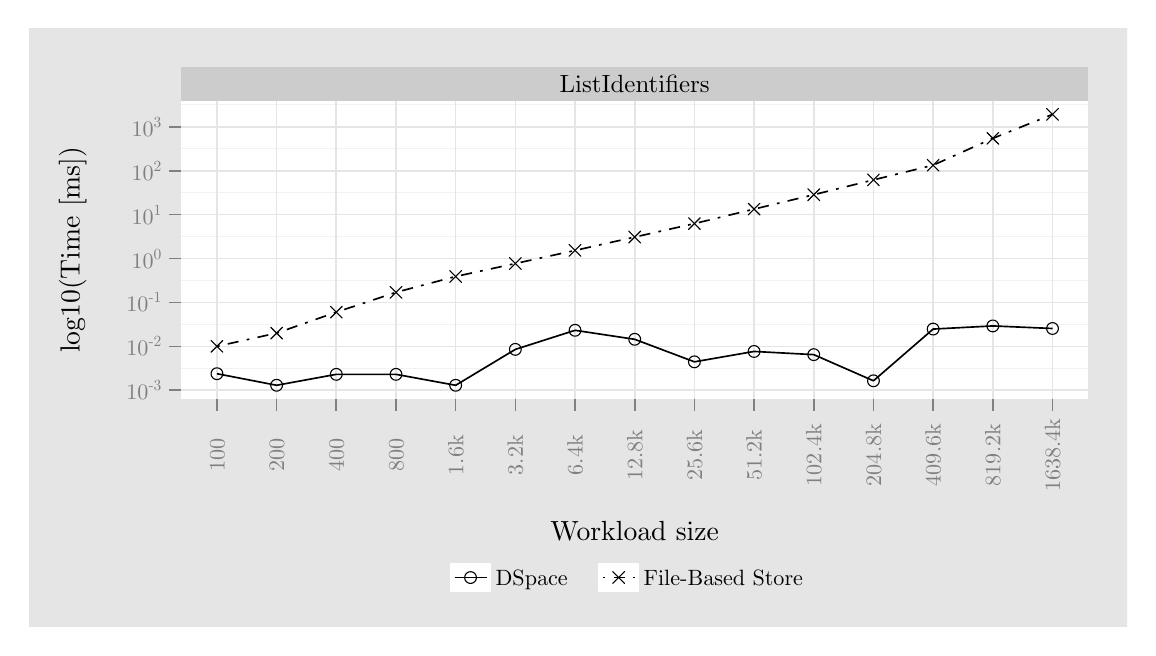
\begin{tikzpicture}[x=1pt,y=1pt]
\definecolor[named]{fillColor}{rgb}{1.00,1.00,1.00}
\path[use as bounding box,fill=fillColor,fill opacity=0.00] (0,0) rectangle (397.48,216.81);
\begin{scope}
\path[clip] (  0.00,  0.00) rectangle (397.48,216.81);
\definecolor[named]{drawColor}{rgb}{1.00,1.00,1.00}
\definecolor[named]{fillColor}{rgb}{0.90,0.90,0.90}

\path[draw=drawColor,line width= 0.6pt,line join=round,line cap=round,fill=fillColor] (  0.00,  0.00) rectangle (397.48,216.81);
\end{scope}
\begin{scope}
\path[clip] ( 55.45, 82.69) rectangle (383.26,190.36);
\definecolor[named]{fillColor}{rgb}{1.00,1.00,1.00}

\path[fill=fillColor] ( 55.45, 82.69) rectangle (383.26,190.36);
\definecolor[named]{drawColor}{rgb}{0.95,0.95,0.95}

\path[draw=drawColor,line width= 0.3pt,line join=round] ( 55.45, 93.73) --
	(383.26, 93.73);

\path[draw=drawColor,line width= 0.3pt,line join=round] ( 55.45,109.59) --
	(383.26,109.59);

\path[draw=drawColor,line width= 0.3pt,line join=round] ( 55.45,125.45) --
	(383.26,125.45);

\path[draw=drawColor,line width= 0.3pt,line join=round] ( 55.45,141.31) --
	(383.26,141.31);

\path[draw=drawColor,line width= 0.3pt,line join=round] ( 55.45,157.17) --
	(383.26,157.17);

\path[draw=drawColor,line width= 0.3pt,line join=round] ( 55.45,173.03) --
	(383.26,173.03);

\path[draw=drawColor,line width= 0.3pt,line join=round] ( 55.45,188.90) --
	(383.26,188.90);
\definecolor[named]{drawColor}{rgb}{0.90,0.90,0.90}

\path[draw=drawColor,line width= 0.6pt,line join=round] ( 55.45, 85.80) --
	(383.26, 85.80);

\path[draw=drawColor,line width= 0.6pt,line join=round] ( 55.45,101.66) --
	(383.26,101.66);

\path[draw=drawColor,line width= 0.6pt,line join=round] ( 55.45,117.52) --
	(383.26,117.52);

\path[draw=drawColor,line width= 0.6pt,line join=round] ( 55.45,133.38) --
	(383.26,133.38);

\path[draw=drawColor,line width= 0.6pt,line join=round] ( 55.45,149.24) --
	(383.26,149.24);

\path[draw=drawColor,line width= 0.6pt,line join=round] ( 55.45,165.10) --
	(383.26,165.10);

\path[draw=drawColor,line width= 0.6pt,line join=round] ( 55.45,180.96) --
	(383.26,180.96);

\path[draw=drawColor,line width= 0.6pt,line join=round] ( 68.39, 82.69) --
	( 68.39,190.36);

\path[draw=drawColor,line width= 0.6pt,line join=round] ( 89.95, 82.69) --
	( 89.95,190.36);

\path[draw=drawColor,line width= 0.6pt,line join=round] (111.52, 82.69) --
	(111.52,190.36);

\path[draw=drawColor,line width= 0.6pt,line join=round] (133.09, 82.69) --
	(133.09,190.36);

\path[draw=drawColor,line width= 0.6pt,line join=round] (154.65, 82.69) --
	(154.65,190.36);

\path[draw=drawColor,line width= 0.6pt,line join=round] (176.22, 82.69) --
	(176.22,190.36);

\path[draw=drawColor,line width= 0.6pt,line join=round] (197.79, 82.69) --
	(197.79,190.36);

\path[draw=drawColor,line width= 0.6pt,line join=round] (219.35, 82.69) --
	(219.35,190.36);

\path[draw=drawColor,line width= 0.6pt,line join=round] (240.92, 82.69) --
	(240.92,190.36);

\path[draw=drawColor,line width= 0.6pt,line join=round] (262.49, 82.69) --
	(262.49,190.36);

\path[draw=drawColor,line width= 0.6pt,line join=round] (284.05, 82.69) --
	(284.05,190.36);

\path[draw=drawColor,line width= 0.6pt,line join=round] (305.62, 82.69) --
	(305.62,190.36);

\path[draw=drawColor,line width= 0.6pt,line join=round] (327.19, 82.69) --
	(327.19,190.36);

\path[draw=drawColor,line width= 0.6pt,line join=round] (348.75, 82.69) --
	(348.75,190.36);

\path[draw=drawColor,line width= 0.6pt,line join=round] (370.32, 82.69) --
	(370.32,190.36);
\definecolor[named]{drawColor}{rgb}{0.00,0.00,0.00}

\path[draw=drawColor,line width= 0.6pt,line join=round] ( 68.39, 91.77) --
	( 89.95, 87.59) --
	(111.52, 91.54) --
	(133.09, 91.54) --
	(154.65, 87.58) --
	(176.22,100.56) --
	(197.79,107.45) --
	(219.35,104.20) --
	(240.92, 96.06) --
	(262.49, 99.81) --
	(284.05, 98.66) --
	(305.62, 89.21) --
	(327.19,107.90) --
	(348.75,109.03) --
	(370.32,108.11);

\path[draw=drawColor,line width= 0.6pt,dash pattern=on 1pt off 3pt on 4pt off 3pt ,line join=round] ( 68.39,101.66) --
	( 89.95,106.43) --
	(111.52,114.00) --
	(133.09,121.18) --
	(154.65,126.90) --
	(176.22,131.58) --
	(197.79,136.31) --
	(219.35,141.15) --
	(240.92,146.01) --
	(262.49,151.25) --
	(284.05,156.45) --
	(305.62,161.80) --
	(327.19,167.12) --
	(348.75,176.82) --
	(370.32,185.47);

\path[draw=drawColor,line width= 0.4pt,line join=round,line cap=round] ( 68.39, 91.77) circle (  2.13);

\path[draw=drawColor,line width= 0.4pt,line join=round,line cap=round] ( 89.95, 87.59) circle (  2.13);

\path[draw=drawColor,line width= 0.4pt,line join=round,line cap=round] (111.52, 91.54) circle (  2.13);

\path[draw=drawColor,line width= 0.4pt,line join=round,line cap=round] (133.09, 91.54) circle (  2.13);

\path[draw=drawColor,line width= 0.4pt,line join=round,line cap=round] (154.65, 87.58) circle (  2.13);

\path[draw=drawColor,line width= 0.4pt,line join=round,line cap=round] (176.22,100.56) circle (  2.13);

\path[draw=drawColor,line width= 0.4pt,line join=round,line cap=round] (197.79,107.45) circle (  2.13);

\path[draw=drawColor,line width= 0.4pt,line join=round,line cap=round] (219.35,104.20) circle (  2.13);

\path[draw=drawColor,line width= 0.4pt,line join=round,line cap=round] (240.92, 96.06) circle (  2.13);

\path[draw=drawColor,line width= 0.4pt,line join=round,line cap=round] (262.49, 99.81) circle (  2.13);

\path[draw=drawColor,line width= 0.4pt,line join=round,line cap=round] (284.05, 98.66) circle (  2.13);

\path[draw=drawColor,line width= 0.4pt,line join=round,line cap=round] (305.62, 89.21) circle (  2.13);

\path[draw=drawColor,line width= 0.4pt,line join=round,line cap=round] (327.19,107.90) circle (  2.13);

\path[draw=drawColor,line width= 0.4pt,line join=round,line cap=round] (348.75,109.03) circle (  2.13);

\path[draw=drawColor,line width= 0.4pt,line join=round,line cap=round] (370.32,108.11) circle (  2.13);

\path[draw=drawColor,line width= 0.4pt,line join=round,line cap=round,fill=fillColor] ( 66.25, 99.53) -- ( 70.52,103.79);

\path[draw=drawColor,line width= 0.4pt,line join=round,line cap=round,fill=fillColor] ( 66.25,103.79) -- ( 70.52, 99.53);

\path[draw=drawColor,line width= 0.4pt,line join=round,line cap=round,fill=fillColor] ( 87.82,104.30) -- ( 92.09,108.57);

\path[draw=drawColor,line width= 0.4pt,line join=round,line cap=round,fill=fillColor] ( 87.82,108.57) -- ( 92.09,104.30);

\path[draw=drawColor,line width= 0.4pt,line join=round,line cap=round,fill=fillColor] (109.39,111.87) -- (113.66,116.14);

\path[draw=drawColor,line width= 0.4pt,line join=round,line cap=round,fill=fillColor] (109.39,116.14) -- (113.66,111.87);

\path[draw=drawColor,line width= 0.4pt,line join=round,line cap=round,fill=fillColor] (130.95,119.04) -- (135.22,123.31);

\path[draw=drawColor,line width= 0.4pt,line join=round,line cap=round,fill=fillColor] (130.95,123.31) -- (135.22,119.04);

\path[draw=drawColor,line width= 0.4pt,line join=round,line cap=round,fill=fillColor] (152.52,124.76) -- (156.79,129.03);

\path[draw=drawColor,line width= 0.4pt,line join=round,line cap=round,fill=fillColor] (152.52,129.03) -- (156.79,124.76);

\path[draw=drawColor,line width= 0.4pt,line join=round,line cap=round,fill=fillColor] (174.09,129.45) -- (178.35,133.72);

\path[draw=drawColor,line width= 0.4pt,line join=round,line cap=round,fill=fillColor] (174.09,133.72) -- (178.35,129.45);

\path[draw=drawColor,line width= 0.4pt,line join=round,line cap=round,fill=fillColor] (195.65,134.18) -- (199.92,138.45);

\path[draw=drawColor,line width= 0.4pt,line join=round,line cap=round,fill=fillColor] (195.65,138.45) -- (199.92,134.18);

\path[draw=drawColor,line width= 0.4pt,line join=round,line cap=round,fill=fillColor] (217.22,139.02) -- (221.49,143.29);

\path[draw=drawColor,line width= 0.4pt,line join=round,line cap=round,fill=fillColor] (217.22,143.29) -- (221.49,139.02);

\path[draw=drawColor,line width= 0.4pt,line join=round,line cap=round,fill=fillColor] (238.79,143.87) -- (243.05,148.14);

\path[draw=drawColor,line width= 0.4pt,line join=round,line cap=round,fill=fillColor] (238.79,148.14) -- (243.05,143.87);

\path[draw=drawColor,line width= 0.4pt,line join=round,line cap=round,fill=fillColor] (260.35,149.11) -- (264.62,153.38);

\path[draw=drawColor,line width= 0.4pt,line join=round,line cap=round,fill=fillColor] (260.35,153.38) -- (264.62,149.11);

\path[draw=drawColor,line width= 0.4pt,line join=round,line cap=round,fill=fillColor] (281.92,154.31) -- (286.19,158.58);

\path[draw=drawColor,line width= 0.4pt,line join=round,line cap=round,fill=fillColor] (281.92,158.58) -- (286.19,154.31);

\path[draw=drawColor,line width= 0.4pt,line join=round,line cap=round,fill=fillColor] (303.49,159.66) -- (307.75,163.93);

\path[draw=drawColor,line width= 0.4pt,line join=round,line cap=round,fill=fillColor] (303.49,163.93) -- (307.75,159.66);

\path[draw=drawColor,line width= 0.4pt,line join=round,line cap=round,fill=fillColor] (325.05,164.98) -- (329.32,169.25);

\path[draw=drawColor,line width= 0.4pt,line join=round,line cap=round,fill=fillColor] (325.05,169.25) -- (329.32,164.98);

\path[draw=drawColor,line width= 0.4pt,line join=round,line cap=round,fill=fillColor] (346.62,174.69) -- (350.89,178.96);

\path[draw=drawColor,line width= 0.4pt,line join=round,line cap=round,fill=fillColor] (346.62,178.96) -- (350.89,174.69);

\path[draw=drawColor,line width= 0.4pt,line join=round,line cap=round,fill=fillColor] (368.18,183.33) -- (372.45,187.60);

\path[draw=drawColor,line width= 0.4pt,line join=round,line cap=round,fill=fillColor] (368.18,187.60) -- (372.45,183.33);
\end{scope}
\begin{scope}
\path[clip] (  0.00,  0.00) rectangle (397.48,216.81);
\definecolor[named]{fillColor}{rgb}{0.80,0.80,0.80}

\path[fill=fillColor] ( 55.45,190.36) rectangle (383.26,202.58);
\definecolor[named]{drawColor}{rgb}{0.00,0.00,0.00}

\node[text=drawColor,anchor=base,inner sep=0pt, outer sep=0pt, scale=  0.90] at (219.35,193.37) {ListIdentifiers};
\end{scope}
\begin{scope}
\path[clip] (  0.00,  0.00) rectangle (397.48,216.81);
\definecolor[named]{drawColor}{rgb}{0.50,0.50,0.50}

\node[text=drawColor,anchor=base west,inner sep=0pt, outer sep=0pt, scale=  0.80] at ( 35.67, 82.37) {10};

\node[text=drawColor,anchor=base west,inner sep=0pt, outer sep=0pt, scale=  0.56] at ( 43.67, 85.64) {-};

\node[text=drawColor,anchor=base west,inner sep=0pt, outer sep=0pt, scale=  0.56] at ( 45.54, 85.64) {3};

\node[text=drawColor,anchor=base west,inner sep=0pt, outer sep=0pt, scale=  0.80] at ( 35.67, 98.23) {10};

\node[text=drawColor,anchor=base west,inner sep=0pt, outer sep=0pt, scale=  0.56] at ( 43.67,101.50) {-};

\node[text=drawColor,anchor=base west,inner sep=0pt, outer sep=0pt, scale=  0.56] at ( 45.54,101.50) {2};

\node[text=drawColor,anchor=base west,inner sep=0pt, outer sep=0pt, scale=  0.80] at ( 35.67,114.09) {10};

\node[text=drawColor,anchor=base west,inner sep=0pt, outer sep=0pt, scale=  0.56] at ( 43.67,117.36) {-};

\node[text=drawColor,anchor=base west,inner sep=0pt, outer sep=0pt, scale=  0.56] at ( 45.54,117.36) {1};

\node[text=drawColor,anchor=base west,inner sep=0pt, outer sep=0pt, scale=  0.80] at ( 37.54,129.95) {10};

\node[text=drawColor,anchor=base west,inner sep=0pt, outer sep=0pt, scale=  0.56] at ( 45.54,133.22) {0};

\node[text=drawColor,anchor=base west,inner sep=0pt, outer sep=0pt, scale=  0.80] at ( 37.54,145.81) {10};

\node[text=drawColor,anchor=base west,inner sep=0pt, outer sep=0pt, scale=  0.56] at ( 45.54,149.08) {1};

\node[text=drawColor,anchor=base west,inner sep=0pt, outer sep=0pt, scale=  0.80] at ( 37.54,161.67) {10};

\node[text=drawColor,anchor=base west,inner sep=0pt, outer sep=0pt, scale=  0.56] at ( 45.54,164.94) {2};

\node[text=drawColor,anchor=base west,inner sep=0pt, outer sep=0pt, scale=  0.80] at ( 37.54,177.53) {10};

\node[text=drawColor,anchor=base west,inner sep=0pt, outer sep=0pt, scale=  0.56] at ( 45.54,180.80) {3};
\end{scope}
\begin{scope}
\path[clip] (  0.00,  0.00) rectangle (397.48,216.81);
\definecolor[named]{drawColor}{rgb}{0.50,0.50,0.50}

\path[draw=drawColor,line width= 0.6pt,line join=round] ( 51.18, 85.80) --
	( 55.45, 85.80);

\path[draw=drawColor,line width= 0.6pt,line join=round] ( 51.18,101.66) --
	( 55.45,101.66);

\path[draw=drawColor,line width= 0.6pt,line join=round] ( 51.18,117.52) --
	( 55.45,117.52);

\path[draw=drawColor,line width= 0.6pt,line join=round] ( 51.18,133.38) --
	( 55.45,133.38);

\path[draw=drawColor,line width= 0.6pt,line join=round] ( 51.18,149.24) --
	( 55.45,149.24);

\path[draw=drawColor,line width= 0.6pt,line join=round] ( 51.18,165.10) --
	( 55.45,165.10);

\path[draw=drawColor,line width= 0.6pt,line join=round] ( 51.18,180.96) --
	( 55.45,180.96);
\end{scope}
\begin{scope}
\path[clip] (  0.00,  0.00) rectangle (397.48,216.81);
\definecolor[named]{drawColor}{rgb}{0.50,0.50,0.50}

\path[draw=drawColor,line width= 0.6pt,line join=round] ( 68.39, 78.42) --
	( 68.39, 82.69);

\path[draw=drawColor,line width= 0.6pt,line join=round] ( 89.95, 78.42) --
	( 89.95, 82.69);

\path[draw=drawColor,line width= 0.6pt,line join=round] (111.52, 78.42) --
	(111.52, 82.69);

\path[draw=drawColor,line width= 0.6pt,line join=round] (133.09, 78.42) --
	(133.09, 82.69);

\path[draw=drawColor,line width= 0.6pt,line join=round] (154.65, 78.42) --
	(154.65, 82.69);

\path[draw=drawColor,line width= 0.6pt,line join=round] (176.22, 78.42) --
	(176.22, 82.69);

\path[draw=drawColor,line width= 0.6pt,line join=round] (197.79, 78.42) --
	(197.79, 82.69);

\path[draw=drawColor,line width= 0.6pt,line join=round] (219.35, 78.42) --
	(219.35, 82.69);

\path[draw=drawColor,line width= 0.6pt,line join=round] (240.92, 78.42) --
	(240.92, 82.69);

\path[draw=drawColor,line width= 0.6pt,line join=round] (262.49, 78.42) --
	(262.49, 82.69);

\path[draw=drawColor,line width= 0.6pt,line join=round] (284.05, 78.42) --
	(284.05, 82.69);

\path[draw=drawColor,line width= 0.6pt,line join=round] (305.62, 78.42) --
	(305.62, 82.69);

\path[draw=drawColor,line width= 0.6pt,line join=round] (327.19, 78.42) --
	(327.19, 82.69);

\path[draw=drawColor,line width= 0.6pt,line join=round] (348.75, 78.42) --
	(348.75, 82.69);

\path[draw=drawColor,line width= 0.6pt,line join=round] (370.32, 78.42) --
	(370.32, 82.69);
\end{scope}
\begin{scope}
\path[clip] (  0.00,  0.00) rectangle (397.48,216.81);
\definecolor[named]{drawColor}{rgb}{0.50,0.50,0.50}

\node[text=drawColor,rotate= 90.00,anchor=base,inner sep=0pt, outer sep=0pt, scale=  0.80] at ( 71.14, 62.36) {100};

\node[text=drawColor,rotate= 90.00,anchor=base,inner sep=0pt, outer sep=0pt, scale=  0.80] at ( 92.71, 62.36) {200};

\node[text=drawColor,rotate= 90.00,anchor=base,inner sep=0pt, outer sep=0pt, scale=  0.80] at (114.28, 62.36) {400};

\node[text=drawColor,rotate= 90.00,anchor=base,inner sep=0pt, outer sep=0pt, scale=  0.80] at (135.84, 62.36) {800};

\node[text=drawColor,rotate= 90.00,anchor=base,inner sep=0pt, outer sep=0pt, scale=  0.80] at (157.41, 62.36) {1.6k};

\node[text=drawColor,rotate= 90.00,anchor=base,inner sep=0pt, outer sep=0pt, scale=  0.80] at (178.98, 62.36) {3.2k};

\node[text=drawColor,rotate= 90.00,anchor=base,inner sep=0pt, outer sep=0pt, scale=  0.80] at (200.54, 62.36) {6.4k};

\node[text=drawColor,rotate= 90.00,anchor=base,inner sep=0pt, outer sep=0pt, scale=  0.80] at (222.11, 62.36) {12.8k};

\node[text=drawColor,rotate= 90.00,anchor=base,inner sep=0pt, outer sep=0pt, scale=  0.80] at (243.67, 62.36) {25.6k};

\node[text=drawColor,rotate= 90.00,anchor=base,inner sep=0pt, outer sep=0pt, scale=  0.80] at (265.24, 62.36) {51.2k};

\node[text=drawColor,rotate= 90.00,anchor=base,inner sep=0pt, outer sep=0pt, scale=  0.80] at (286.81, 62.36) {102.4k};

\node[text=drawColor,rotate= 90.00,anchor=base,inner sep=0pt, outer sep=0pt, scale=  0.80] at (308.37, 62.36) {204.8k};

\node[text=drawColor,rotate= 90.00,anchor=base,inner sep=0pt, outer sep=0pt, scale=  0.80] at (329.94, 62.36) {409.6k};

\node[text=drawColor,rotate= 90.00,anchor=base,inner sep=0pt, outer sep=0pt, scale=  0.80] at (351.51, 62.36) {819.2k};

\node[text=drawColor,rotate= 90.00,anchor=base,inner sep=0pt, outer sep=0pt, scale=  0.80] at (373.07, 62.36) {1638.4k};
\end{scope}
\begin{scope}
\path[clip] (  0.00,  0.00) rectangle (397.48,216.81);
\definecolor[named]{drawColor}{rgb}{0.00,0.00,0.00}

\node[text=drawColor,anchor=base,inner sep=0pt, outer sep=0pt, scale=  1.00] at (219.35, 31.41) {Workload size};
\end{scope}
\begin{scope}
\path[clip] (  0.00,  0.00) rectangle (397.48,216.81);
\definecolor[named]{drawColor}{rgb}{0.00,0.00,0.00}

\node[text=drawColor,rotate= 90.00,anchor=base,inner sep=0pt, outer sep=0pt, scale=  1.00] at ( 18.80,136.53) {log10(Time [ms])};
\end{scope}
\begin{scope}
\path[clip] (  0.00,  0.00) rectangle (397.48,216.81);
\definecolor[named]{fillColor}{rgb}{0.90,0.90,0.90}

\path[fill=fillColor] (144.93,  8.87) rectangle (293.78, 27.36);
\end{scope}
\begin{scope}
\path[clip] (  0.00,  0.00) rectangle (397.48,216.81);
\definecolor[named]{drawColor}{rgb}{1.00,1.00,1.00}
\definecolor[named]{fillColor}{rgb}{1.00,1.00,1.00}

\path[draw=drawColor,line width= 0.6pt,line join=round,line cap=round,fill=fillColor] (152.81, 13.14) rectangle (167.26, 23.09);
\end{scope}
\begin{scope}
\path[clip] (  0.00,  0.00) rectangle (397.48,216.81);
\definecolor[named]{drawColor}{rgb}{0.00,0.00,0.00}

\path[draw=drawColor,line width= 0.6pt,line join=round] (154.25, 18.11) -- (165.82, 18.11);
\end{scope}
\begin{scope}
\path[clip] (  0.00,  0.00) rectangle (397.48,216.81);
\definecolor[named]{drawColor}{rgb}{0.00,0.00,0.00}

\path[draw=drawColor,line width= 0.4pt,line join=round,line cap=round] (160.03, 18.11) circle (  2.13);
\end{scope}
\begin{scope}
\path[clip] (  0.00,  0.00) rectangle (397.48,216.81);
\definecolor[named]{drawColor}{rgb}{1.00,1.00,1.00}
\definecolor[named]{fillColor}{rgb}{1.00,1.00,1.00}

\path[draw=drawColor,line width= 0.6pt,line join=round,line cap=round,fill=fillColor] (206.31, 13.14) rectangle (220.77, 23.09);
\end{scope}
\begin{scope}
\path[clip] (  0.00,  0.00) rectangle (397.48,216.81);
\definecolor[named]{drawColor}{rgb}{0.00,0.00,0.00}

\path[draw=drawColor,line width= 0.6pt,dash pattern=on 1pt off 3pt on 4pt off 3pt ,line join=round] (207.76, 18.11) -- (219.32, 18.11);
\end{scope}
\begin{scope}
\path[clip] (  0.00,  0.00) rectangle (397.48,216.81);
\definecolor[named]{drawColor}{rgb}{0.00,0.00,0.00}
\definecolor[named]{fillColor}{rgb}{1.00,1.00,1.00}

\path[draw=drawColor,line width= 0.4pt,line join=round,line cap=round,fill=fillColor] (211.41, 15.98) -- (215.67, 20.25);

\path[draw=drawColor,line width= 0.4pt,line join=round,line cap=round,fill=fillColor] (211.41, 20.25) -- (215.67, 15.98);
\end{scope}
\begin{scope}
\path[clip] (  0.00,  0.00) rectangle (397.48,216.81);
\definecolor[named]{drawColor}{rgb}{0.00,0.00,0.00}

\node[text=drawColor,anchor=base west,inner sep=0pt, outer sep=0pt, scale=  0.80] at (169.07, 15.36) {DSpace $\;\;\;$};
\end{scope}
\begin{scope}
\path[clip] (  0.00,  0.00) rectangle (397.48,216.81);
\definecolor[named]{drawColor}{rgb}{0.00,0.00,0.00}

\node[text=drawColor,anchor=base west,inner sep=0pt, outer sep=0pt, scale=  0.80] at (222.57, 15.36) {File-Based Store $\;\;\;$};
\end{scope}
\end{tikzpicture}
